\chapter{РАЗРАБОТКА ПРОГРАММНОГО ОБЕСПЕЧЕНИЯ}

\section{Выбор технологий}

\subsection{Библиотека проективной геометрии}
К разрабатываемому приложению были поставлены следующие требования: высокая производительность, удобный и кроссплатформенный пользовательский интерфейс, минимум зависимостей. Для выполнения процесса \textbf{Structure From Motion} была выбрана реализация от Криса Суини (\textit{Chris Sweeney}) - библиотека проективной геометрии с открытым исходным кодом \hyperref[itm:theia]{Theia [\ref{itm:theia}]}. Автор библиотеки, исследователь Вашингтонского университета, занимается разработками в области компьютерного зрения и виртуальной реальности, имеет степень Ph.D., а также множество научных публикаций. Выбор именно этой библиотеки обусловлен несколькими причинами: легковесность (не имеет зависимостей от больших библиотек, таких как OpenCV или Boost), узкая специализация и направленность на решение конкретной задачи, реализация на С++, а также очень хорошая и подробная документация.

\subsection{Пользовательский графический интерфейс}
Для написания графического пользовательского интерфейса отлично подходит \hyperref[itm:qt]{$Qt$ [\ref{itm:qt}]}. $Qt$ - это кроссплатформенный инструментарий разработки приложений на языке программирования C++. $Qt$ позволяет запускать написанное с его помощью программное обеспечение в большинстве современных операционных систем (\textit{Windows, macOS, Linux}) путём простой компиляции программы для каждой операционной системы без изменения исходного кода. Включает в себя множество классов для работы с сетью, базами данных, также предоставлены обширные инструменты по быстрому и удобному созданию интерфейсов. Использует Metaobject-компилятор, который компилирует программы написанные на $Qt$ в C++ код, таким образом расширяя функционал и возможности языка C++. $Qt$ добавляет очень удобные обёртки для STL контейнеров, такие как: QString, QArray, QList, QLinkedList, QStack, QQueue, QMap, QSet и другие.$Qt$ состоит из таких основных модулей как: Qt Core, Qt GUI, Qt QML, Qt Network, Qt SQL, Qt WebEngine и др. Виджеты включают в себя набор таких компонентов как: кнопки, прогресс бары, переключатели, чекбоксы - исчерпывающий набор для создания GUI.

В комплекте с $Qt$ идёт собственная интегрированная среда разработки QtCreator а также Qt Designer, который позволяет создавать интерфейс, просто перетягивая и компонуя виджеты и компоненты на форме, а после описывая для них контроллеры, отвечающие за логику. 

\subsection{Система сборки}
В качестве системы сборки мной был выбран Cmake. Cmake - это кроссплатформеная, бесплатная и свободно распространяемая система управлением процессами сборки программного обеспечения. Поддерживает иерархическую структуру и вложенные структуры. Позволяет описать все зависимости проекта и правила для их поиска и сборки. Основным достоинством является кэширование файлов, включённое по умолчанию, что позволяет значительно увеличить скорость сборки, путем перекомпилирования только изменённых файлов, а оставшиеся брать из кэша. Это является очень критичным для приложений написанных на C++, для которых время компиляции может занимать до пяти минут.

Для описания сборки в директории требуется создать CMakeLists.txt файл в котором перечислить список файлов которые нужно скомпилировать, а также указать ссылки на библиотеки и имя цели, которое в дальнейшем будет использоваться для запуска собранного исполняемого файла.

После завершения своей работы cmake генерирует специальный Makefile который используется стандартный командой сборки для C++ приложений make.

\subsection{Стиль кода}
При разработке приложения было решено придерживаться стиля кода, принятого в компании Google. Google C++ Style Guide - cамый популярный справочник по стилю, набор правил и советов по написанию чистого, читаемого и расширяемого кода на C++ от компании Google. Для того чтобы точно придерживаться этих правил я использовал cpplint - скрипт, который с помощью набора регулярных выражений сканирует все файлы проекта и проверяет выполнение правил, выводит ошибки в удобном и понятном виде.

\section{Разработка алгоритма поиска}
Итак, после выполнения всех этапов Structure From Motion мы имеем 3D модель - реконструкцию поверхности. Модель представляет из себя набор точек пространства с известными для них GPS координатами. Цель алгоритма - найти на построенной 3D карте расположение нового снимка. Предполагается, что на снимке присутствует та же область пространства, что и в модели, иначе ничего найдено не будет. Также снимок должен быть не из исходного датасета, то есть оличный от тех, на основе которых строилась модель. Иначе поиск не будет иметь смысла. Следующая задача алгоритма - найти геометрическое преобразование и с его помощью определить точные координаты точки пространства из которой был сделан искомый снимок.

Для осуществления поиска по модели вместе с каждой 3D точкой сохраняется набор дескрипторов всех особых точек соответствующих этой, реальной точке. 


\vspace{1em}
В итоге получается следующий алгоритм:
\begin{enumerate}
    \item На вход поступает очередной снимок;
    \item Находим ключевые точки и извлекаем соответствующие им дескрипторы;
    \item Сравниваем полученные дескрипторы с сохранёнными в модели;
    \item Находим камеру из исходного датасета, для которой получили наилучшее сопоставление;
    \item Находим геометрическое преобразование, с помощью которого искомый снимок проецируется на \quotes{лучшую} камеру;
    \item По известным GPS-координатам исходной камеры и геометрическому преобразованию находим местоположение искомой камеры.
\end{enumerate}

\vspace{1em}
Также, кроме одной камеры, возможно получение всей области, на которую накладывается искомый снимок.

\section{Приложение для построения реконструкции}

\begin{figure}[h]
    \centering
    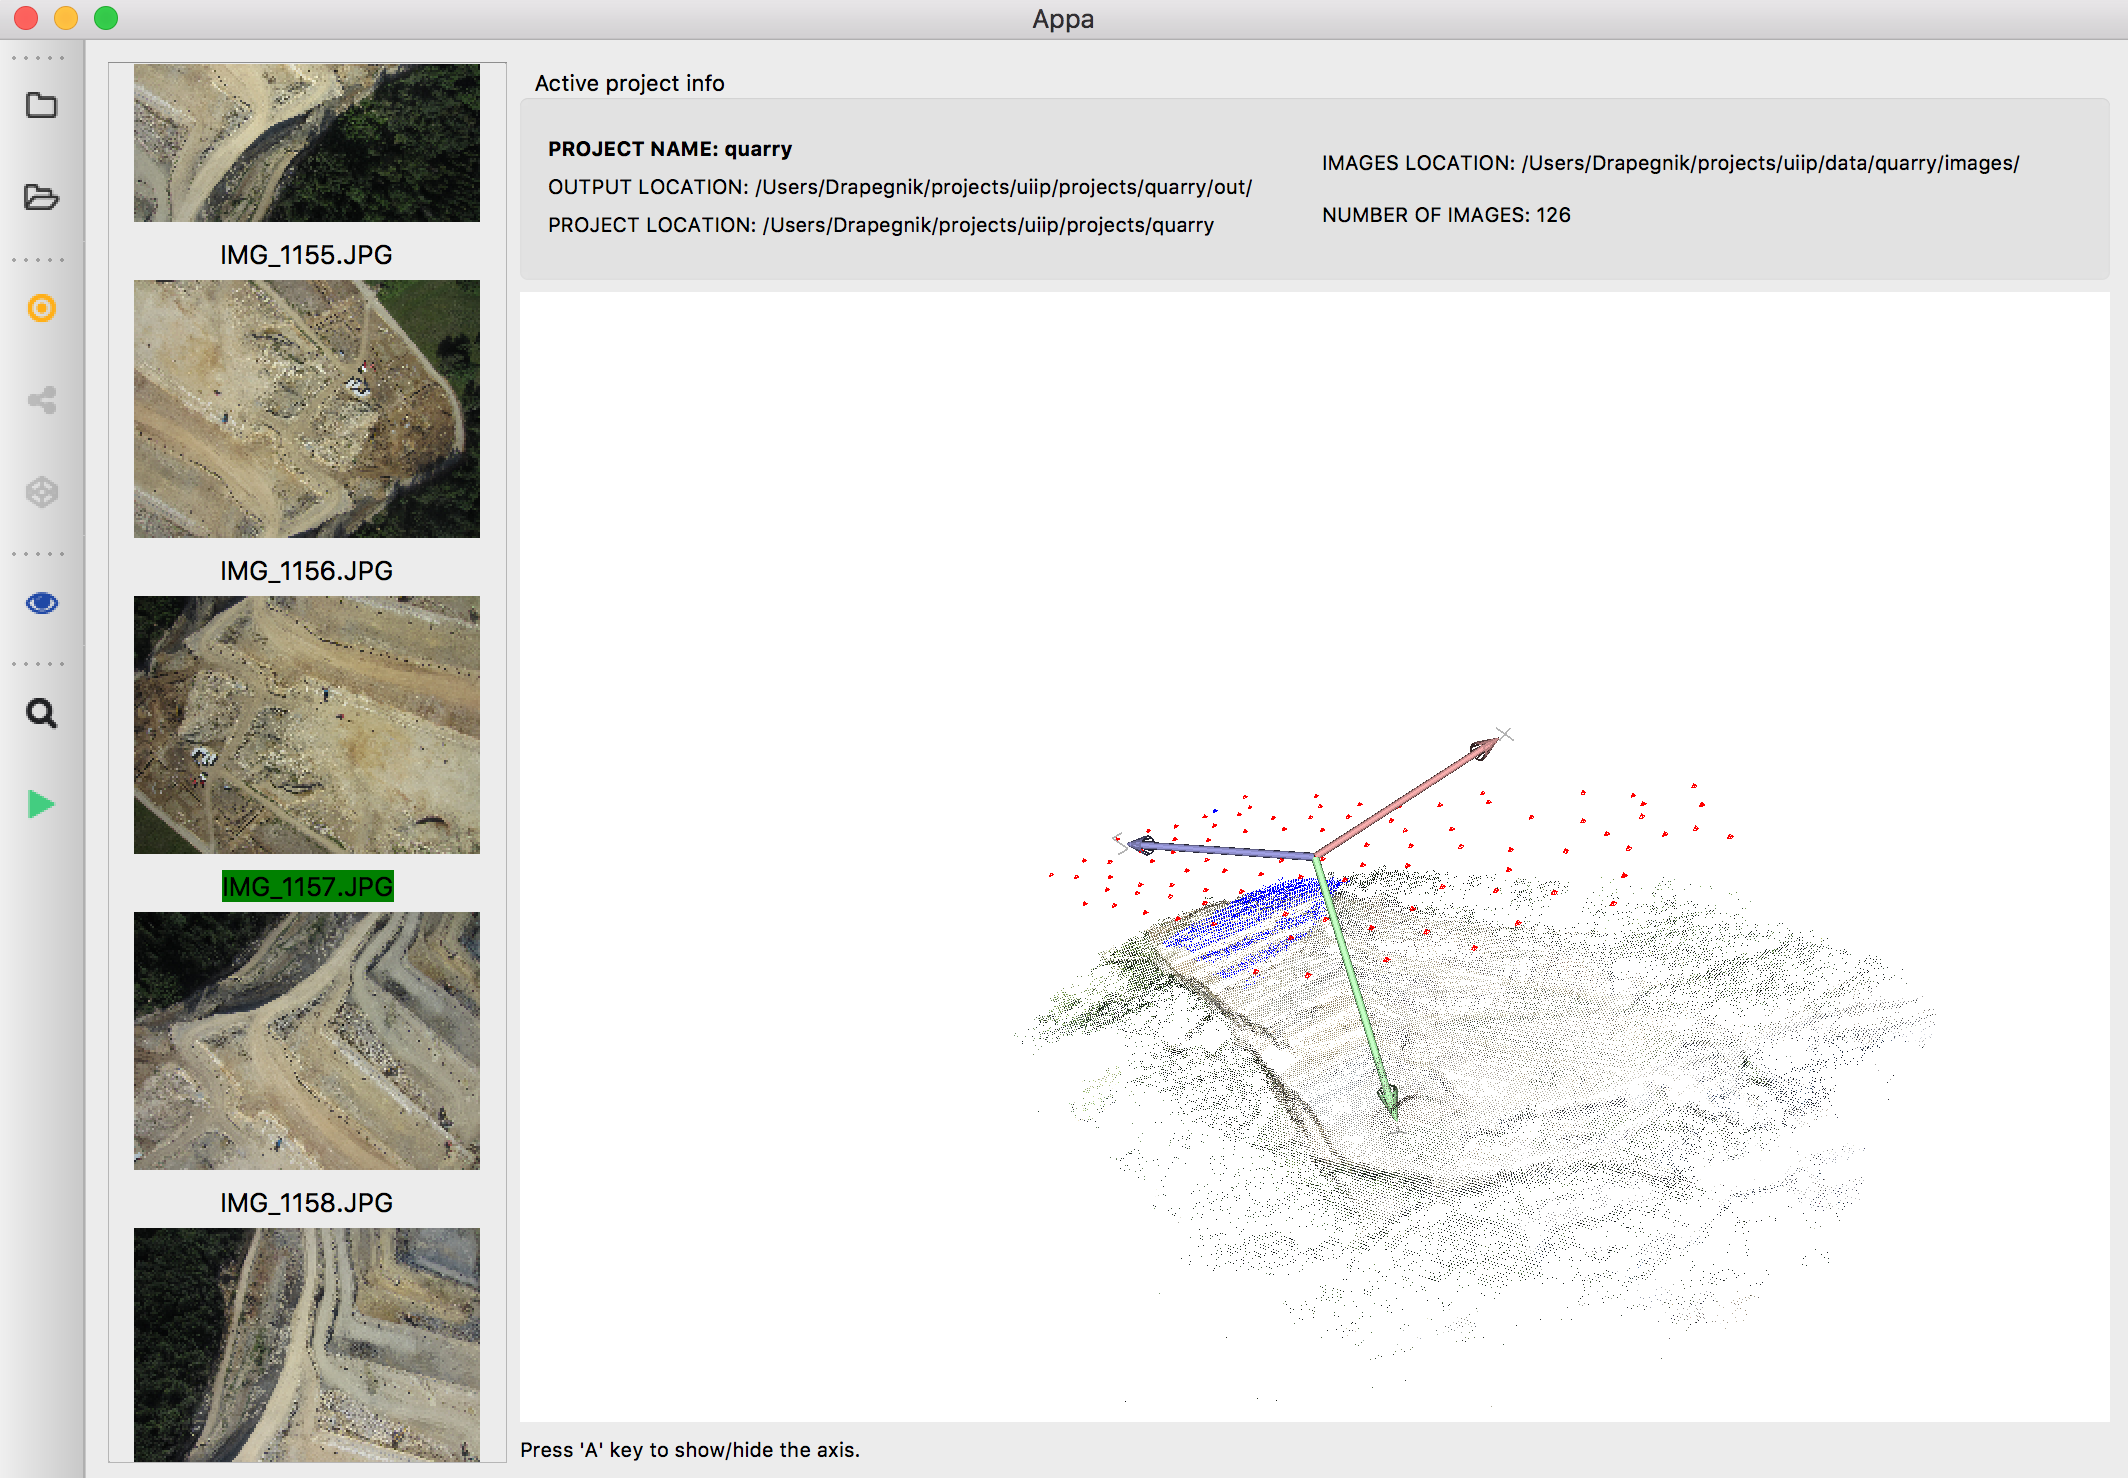
\includegraphics[width=1\textwidth]{appa.png}
    \caption{Приложение для построения и визуализации 3D моделей, осуществления поиска по ним}
    \label{fig:appa}
\end{figure}

На рисунке \ref{fig:appa} представлен интерфейс разработанного приложения. Модель - швейцарский карьер построенный на датасете снятом с помощью беспилотного летательного аппарата. Датасет был найден в одном из открытых источников.

\vspace{1em}
В приложении реализован следующий функционал:
\begin{itemize}
    \item создание нового / открытие существующего проекта;
    \item просмотр датасета текущего проекта;
    \item извлечение ключевых точек;
    \item построение модели;
    \item визуализация модели;
    \item поиск по построенной модели.
\end{itemize}

\vspace{1em}
Рассмотрим функционал приложения подробнее. При создании проекта надо ввести имя проекта, путь к директории с изображениями и директорию для проекта. В этой директории будет создан конфигурационный файл содержащий всю информацию о проекте, пути, настройки и параметры. С этим файлом и будет в будущем ассоциирован проект. Соответственно для открытия проекта требуется открыть папку содержащую этот конфигурационный файл. При визуализации модели, красным отрисовываются положения исходных камер с которых видны ключевые точки. При выборе изображений на боковой панели слева точки выбранного изображения, которые попали в конечную модель подсвечиваются синим (см. рисунок \ref{fig:appa}).

При построении модели можно настроить такие параметры как: количество потоков, в которых будет выполнятся каждая часть процесса Structure From Motion, тип дескриптора и детектора (поддерживаются рассмотренный ранее \hyperref[itm:sift]{SIFT [\ref{itm:sift}]}, а также AKAZE), стратегия сопоставления снимков (Brute Force или Cascade Hashing). Остальные настройки касаются внутренних и внешних параметров камеры. (см. рисунок \ref{fig:appa-options}).

После построения модели её также можно сохранить в файловой системе, по умолчанию в папку текущего проекта. Благодаря этому уже построенные модели можно открывать и визуализировать очень быстро. В одном проекте может быть много моделей, выбор текущей активной модели осуществляется при запуске процесса визуализации.

При запуске процесса поиска открывается диалоговое окно, в котором требуется открыть изображение, которое мы собираемся найти на построенной 3D карте. После выполнения поиска ключевые точки модели сопоставленные с искомым снимком подсвечиваются красным. Таким образом можно определить координаты искомого снимка, так как координаты для изображений составляющих карту известны. Рассматривая производительность: поиск на датасете из $127$ снимков, при извлечении порядка $5000$ ключевых точек на каждом изображении осуществляется, в среднем, за $40-50$ секунд.

\section{Выводы}

В этой главе была представлена проделанная практическая работа. Проанализированы новые технологии и решения. Получен результат работы - рабочее приложение для построения 3D модели и поиска по ней.

Анализируя алгоритм и результаты поиска: итоговое время в разы лучше полученного экспериментально в начале исследований. Но этого всё ещё недостаточно, для стабильной работы в реальном времени на борту беспилотного летательного аппарата. Требуется оптимизация и доработка алгоритма поиска.

\begin{figure}[h]
    \centering
    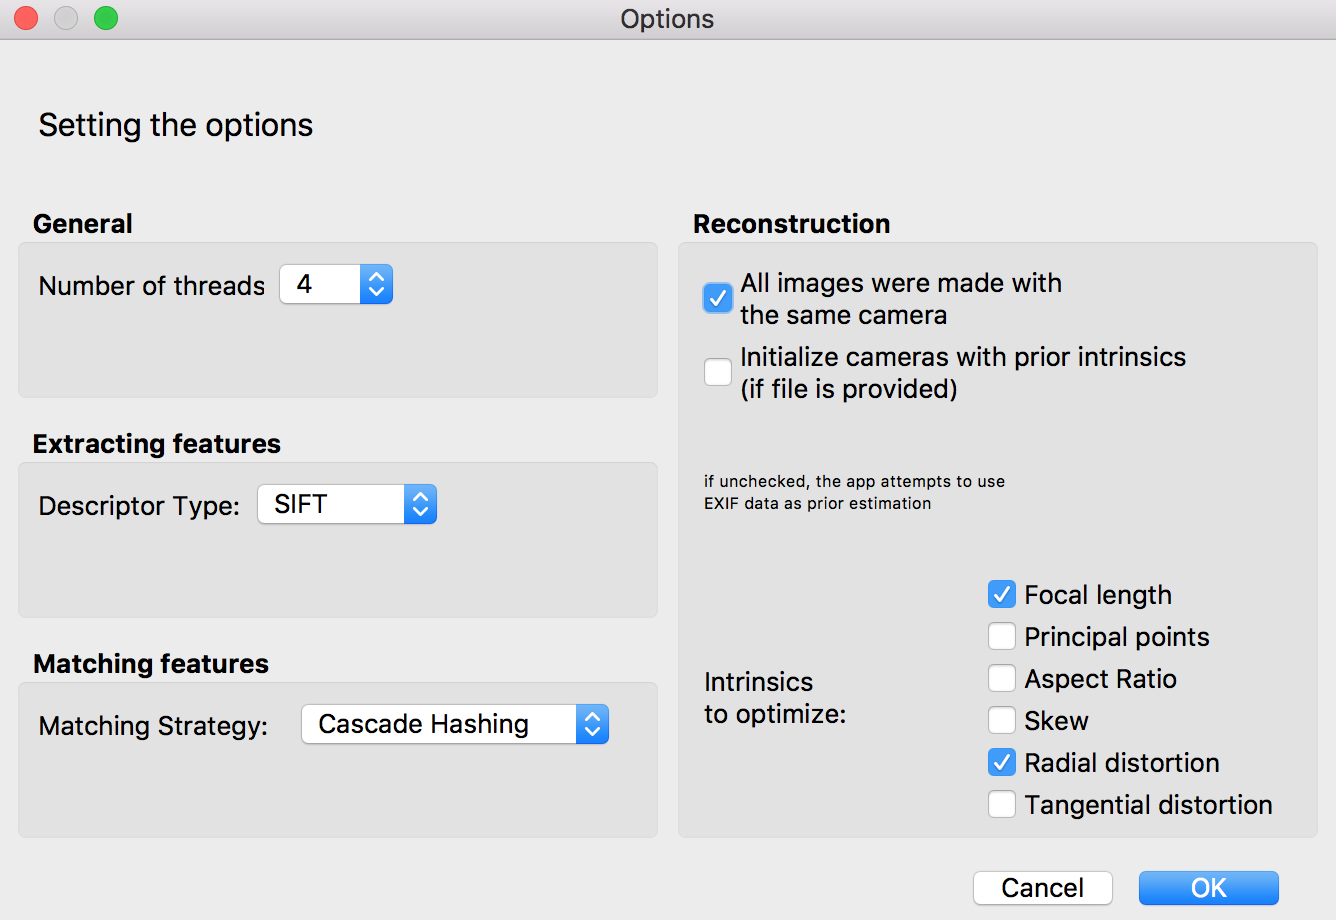
\includegraphics[width=0.9\textwidth]{appa-options.png}
    \caption{Различные параметры построения модели}
    \label{fig:appa-options}
\end{figure}
